%%%%%%%%%%%%%%%%%%%%%%%%%%%%%%%%%%%%%%%%%%%%%%%%%%%%%%%%%%%%%%%%%%%%%%%%%%%%%%%%%%%%%%%%%%%%%%%%%
%
% Document:      DM  product tree
%
%%%%%%%%%%%%%%%%%%%%%%%%%%%%%%%%%%%%%%%%%%%%%%%%%%%%%%%%%%%%%%%%%%%%%%%%%%%%%%
\documentclass{article}
\usepackage{times,layouts}
\usepackage{tikz,hyperref,amsmath}
\usetikzlibrary{positioning,arrows,shapes,decorations.shapes,shapes.arrows}
\usetikzlibrary{backgrounds,calc}
\usepackage[paperwidth=34.800000000000004cm,paperheight=9.18cm,
left=-2mm,top=3mm,bottom=0mm,right=0mm,
noheadfoot,marginparwidth=0pt,includemp=false,
textwidth=30cm,textheight=50mm]{geometry}
\newcommand\showpage{%
\setlayoutscale{0.5}\setlabelfont{\tiny}\printheadingsfalse\printparametersfalse
\currentpage\pagedesign}
\hypersetup{pdftitle={DM products }, pdfsubject={Diagram illustrating the
products in LSST DM }, pdfauthor={ William O'Mullane}}
\tikzstyle{tbox}=[rectangle,text centered, text width=30mm]
\tikzstyle{wbbox}=[rectangle, rounded corners=3pt, draw=black, top color=blue!50!white, bottom color=white, very thick, minimum height=12mm, inner sep=2pt, text centered, text width=30mm]
\tikzstyle{pbox}=[rectangle, rounded corners=3pt, draw=black, top color=yellow!50!white, bottom color=white, very thick, minimum height=35pt, inner sep=2pt, text centered, text width=35mm]
\tikzstyle{pline}=[-, thick]
\begin{document}
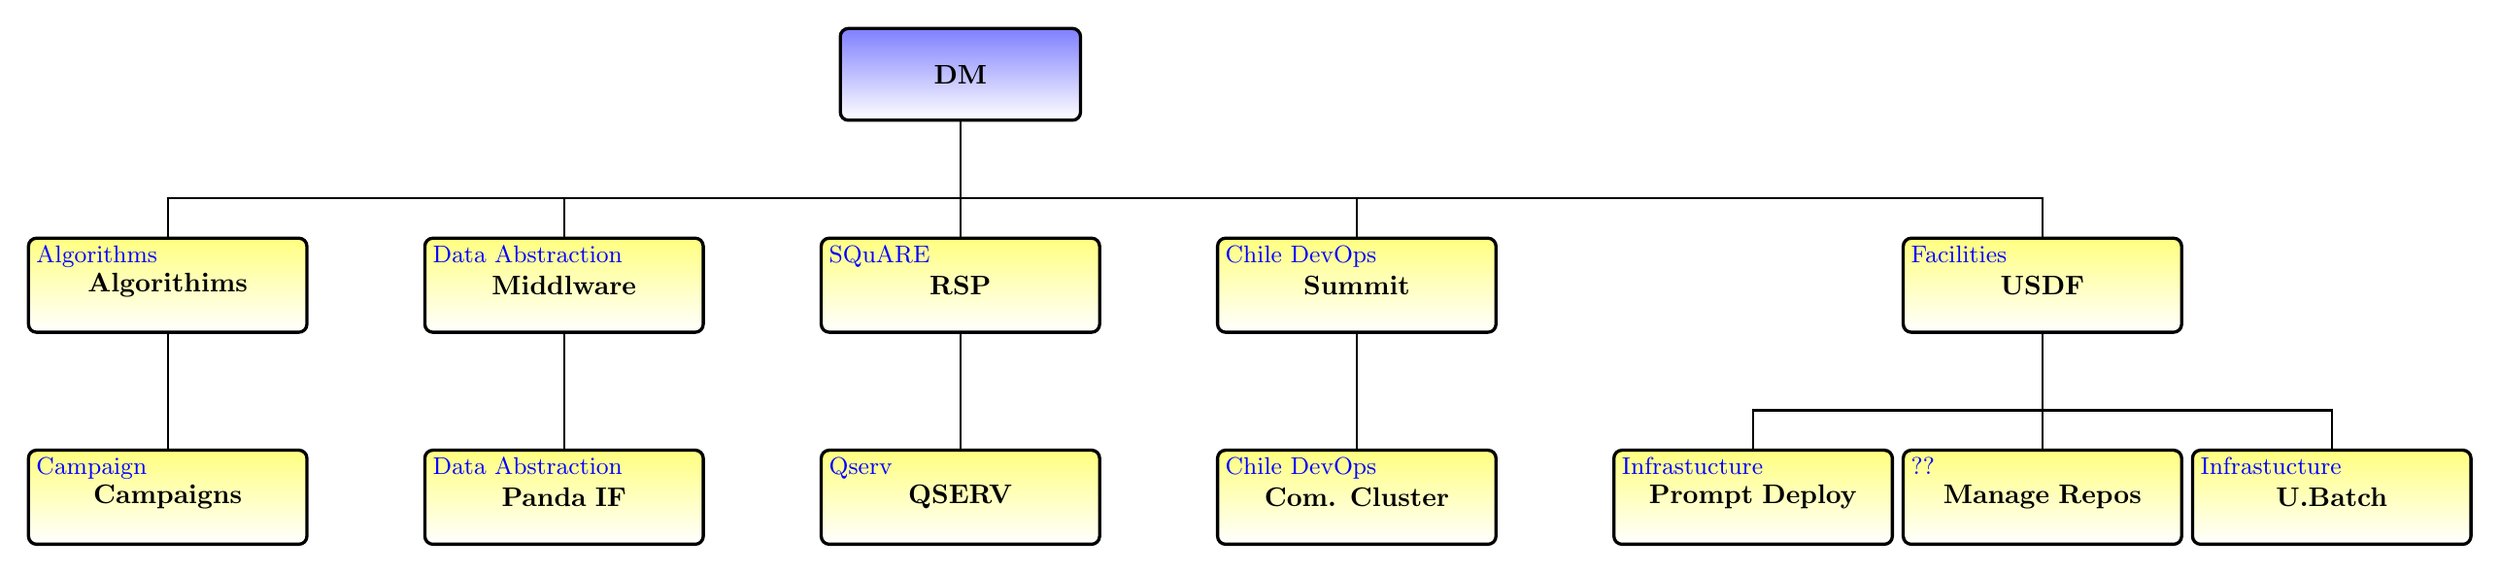
\begin{tikzpicture}[node distance=0mm]
\node (CM) [pbox,] {\textbf{Campaigns} };
\node [below right] at (CM.north west) {\small \color{blue}Campaign} ;
\node (PandaIF) [pbox,right=15mm of CM] {\textbf{Panda IF} };
\node [below right] at (PandaIF.north west) {\small \color{blue}Data Abstraction} ;
\node (QSERV) [pbox,right=15mm of PandaIF] {\textbf{QSERV} };
\node [below right] at (QSERV.north west) {\small \color{blue}Qserv} ;
\node (CC) [pbox,right=15mm of QSERV] {\textbf{Com. Cluster} };
\node [below right] at (CC.north west) {\small \color{blue}Chile DevOps} ;
\node (PPD) [pbox,right=15mm of CC] {\textbf{Prompt Deploy} };
\node [below right] at (PPD.north west) {\small \color{blue}Infrastucture} ;
\node (REPOM) [pbox,right=1mm of PPD] {\textbf{Manage Repos } };
\node [below right] at (REPOM.north west) {\small \color{blue}??} ;
\node (UBATCH) [pbox,right=1mm of REPOM] {\textbf{U.Batch} };
\node [below right] at (UBATCH.north west) {\small \color{blue}Infrastucture} ;
\node (ALP) [pbox,above=15mm of CM] {\textbf{Algorithims} };
\node [below right] at (ALP.north west) {\small \color{blue}Algorithms} ;
\node (MW) [pbox,above=15mm of PandaIF] {\textbf{Middlware} };
\node [below right] at (MW.north west) {\small \color{blue}Data Abstraction} ;
\node (RSP) [pbox,above=15mm of QSERV] {\textbf{RSP} };
\node [below right] at (RSP.north west) {\small \color{blue}SQuARE} ;
\node (SUMMIT) [pbox,above=15mm of CC] {\textbf{Summit} };
\node [below right] at (SUMMIT.north west) {\small \color{blue}Chile DevOps} ;
\node (USDF) [pbox,above=15mm of REPOM] {\textbf{USDF} };
\node [below right] at (USDF.north west) {\small \color{blue}Facilities} ;
 \draw[pline]   (CM.north) -- ++(0.0,0.5) -| (ALP.south) ; 
 \draw[pline]   (PandaIF.north) -- ++(0.0,0.5) -| (MW.south) ; 
 \draw[pline]   (QSERV.north) -- ++(0.0,0.5) -| (RSP.south) ; 
 \draw[pline]   (CC.north) -- ++(0.0,0.5) -| (SUMMIT.south) ; 
 \draw[pline]   (PPD.north) -- ++(0.0,0.5) -| (USDF.south) ; 
 \draw[pline]   (REPOM.north) -- ++(0.0,0.5) -| (USDF.south) ; 
 \draw[pline]   (UBATCH.north) -- ++(0.0,0.5) -| (USDF.south) ; 
\node (DM) [wbbox, above=15mm of RSP]{\textbf{DM}};
 \draw[pline]   (ALP.north) -- ++(0.0,0.5) -| (DM.south) ; 
 \draw[pline]   (MW.north) -- ++(0.0,0.5) -| (DM.south) ; 
 \draw[pline]   (RSP.north) -- ++(0.0,0.5) -| (DM.south) ; 
 \draw[pline]   (SUMMIT.north) -- ++(0.0,0.5) -| (DM.south) ; 
 \draw[pline]   (USDF.north) -- ++(0.0,0.5) -| (DM.south) ; 
\end{tikzpicture}
\end{document}
